\documentclass{beamer}
\usetheme{Berlin}

\title{Systems with a Small Number of
Variables}
\subtitle{Course: Complex Systems Modeling}
\author{Robert Flassig}
\institute{Brandenburg University of Applied Sciences}
\date{\today}

\begin{document}
\begin{frame}
\titlepage
\end{frame}

\begin{frame}
\frametitle{Outline}
\tableofcontents
\end{frame}

\section{Scaling}
\begin{frame}
\frametitle{Motivation for Scaling and Nondimensionalization}

\begin{itemize}
    \item Scaling transforms a model into a \textbf{canonical form} by removing units and redundant parameters.
    \item This highlights the \textbf{essential dynamics} independent of arbitrary units or parameter magnitudes.
    \item Especially useful in \textbf{asymptotic analysis} and \textbf{complex systems modeling}.
\end{itemize}

\vspace{0.3cm}
\textbf{Goal:} Reduce the number of parameters by suitable rescaling of
state variables and time.
\end{frame}

\begin{frame}
\frametitle{Simple ODE Example: Exponential Growth}
\scriptsize
\begin{block}{Model}
\[
\frac{dx}{dt} = r\,x
\]
\end{block}

\small
\begin{itemize}
    \item Exponential growth with rate \(r\).
    \item Introduce scaled variables \(x = \alpha x',\; t = \beta t'\).
\end{itemize}

\medskip
\textbf{Substitute:}
\[
\frac{d(\alpha x')}{d(\beta t')} = r \alpha x'
\;\Rightarrow\;
\frac{dx'}{dt'} = r\,\beta\,x'
\]

\medskip
Choose \(\beta = 1/r\) to remove the parameter:
\[
\boxed{\frac{dx'}{dt'} = x'}
\]

\textbf{Result:} Canonical, dimensionless form.  
Scaling removes units and exposes the fundamental dynamics.
\end{frame}

\begin{frame}
\frametitle{Continuous-Time Logistic Growth Model}

\begin{block}{Original form}
\[
\frac{dx}{dt} = r x \left(1 - \frac{x}{K}\right)
\]
\end{block}

\begin{itemize}
    \item Two parameters: growth rate $r$ and carrying capacity $K$.
    \item In continuous time, we can also rescale \textbf{time}, not only $x$.
\end{itemize}


Apply scaling:
\[
x = \alpha x', \quad t = \beta t'
\]

Substitute and simplify:
\[
\frac{d(\alpha x')}{d(\beta t')} = r \alpha x'\left(1 - \frac{\alpha x'}{K}\right)
\Rightarrow
\frac{dx'}{dt'} = r \beta x' \left(1 - \frac{\alpha x'}{K}\right)
\]
\end{frame}

\begin{frame}
\frametitle{Canonical Logistic Model via Rescaling}

Choose:
\[
\alpha = K, \quad \beta = \frac{1}{r}
\]

Then:
\[
\frac{dx'}{dt'} = x'(1 - x')
\]

\begin{itemize}
    \item All parameters $(r, K)$ are removed.
    \item The resulting equation represents a \textbf{universal canonical form}.
    \item In continuous-time systems, rescaling \textbf{time} removes one additional parameter compared to discrete-time models.
\end{itemize}

\vspace{0.3cm}
\textbf{Interpretation:}  
Changing $r$ or $K$ only stretches trajectories along the time or $x$ axes —  
the qualitative dynamics remain invariant.
\end{frame}

\subsection{Exercises}

\begin{frame}
\frametitle{Exercise: Rescale Quadratic ODE}

Simplify the following differential equation by variable rescaling:
\[
\frac{dx}{dt} = a x^{2} + b x + c
\]

\textbf{Tasks}
\begin{itemize}
  \item (i) Shift \(x\) to remove the linear term.
  \item (ii) Rescale \(x,t\) to eliminate parameters.
  \item (iii) Write the canonical parameter-free form and mention the special case when the shift constant vanishes.
\end{itemize}

\textbf{Hint:} After shifting, you obtain an equation of the form
\[
\dot{y} = a y^2 + d, \qquad d = c - \frac{b^2}{4a}.
\]
\end{frame}

\begin{frame}
\frametitle{Exercise: Rescale Reciprocal+Constant ODE}

Simplify the following ODE by variable rescaling (assume \(a>0,\; b>0\)):
\[
\frac{dx}{dt} = \frac{a}{x} + b
\]

\textbf{Tasks}
\begin{itemize}
  \item (i) Propose the substitutions \(x=\alpha x'\), \(t=\beta t'\).
  \item (ii) Determine \(\alpha,\beta\) so that the coefficients become unity.
  \item (iii) Derive the resulting canonical form.
\end{itemize}
\end{frame}

\subsection{Solutions}

\begin{frame}
\frametitle{Solution: Quadratic ODE}
\small
Given \(\dot x = a x^2 + b x + c\).

\textbf{1. Shift:}
\[
x = y - \frac{b}{2a} \;\Rightarrow\; \dot y = a y^2 + d, 
\quad d := c - \frac{b^2}{4a}.
\]

\textbf{2. Rescale:}
\[
y = \kappa u, \quad t = \frac{\tau}{\gamma}, 
\quad \text{where} \quad 
\kappa = \sqrt{\frac{|d|}{a}}, \;\; \gamma = a\kappa = \sqrt{a|d|}.
\]

\textbf{3. Substitute:}
\[
\frac{dy}{dt} = a y^2 + d 
\;\Rightarrow\;
\frac{du}{d\tau} = u^2 + \operatorname{sgn}(d).
\]

\textbf{Special case:} \(d = 0 \Rightarrow \dot y = a y^2,\; t' = a t \Rightarrow \tfrac{dy}{dt'} = y^2.\)

\textbf{Canonical forms:}
\[
\boxed{u' = u^2 + 1}, \quad
\boxed{u' = u^2 - 1}, \quad
\boxed{y' = y^2}\; (d=0)
\]
\end{frame}

\begin{frame}
\frametitle{Solution: Reciprocal+Constant ODE}
\small
Given \(\dot x = \dfrac{a}{x} + b\), with \(a>0,\; b>0\).

\textbf{1. Substitute:}
\[
x=\alpha x',\; t=\beta t'
\quad \Rightarrow \quad
\frac{\alpha\,dx'}{\beta\,dt'} = \frac{a}{\alpha x'} + b
\]

\textbf{2. Simplify:}
\[
\frac{dx'}{dt'} = 
\frac{\beta a}{\alpha^{2}}\frac{1}{x'} + \frac{\beta b}{\alpha}
\]

\textbf{3. Choose scales:}
\[
\frac{\beta a}{\alpha^{2}}=1,\quad \frac{\beta b}{\alpha}=1
\;\Rightarrow\;
\alpha = \frac{a}{b},\quad \beta = \frac{a}{b^{2}}.
\]

\textbf{4. Canonical form:}
\[
x=\frac{a}{b}x',\quad t=\frac{a}{b^{2}}t'
\quad \Longrightarrow \quad
\boxed{\frac{dx'}{dt'} = \frac{1}{x'} + 1.}
\]
\end{frame}



\subsection{Conceptual Summary}
\begin{frame}
%\frametitle{Conceptual Summary}

\begin{itemize}
    \item Scaling transforms physical models into \textbf{dimensionless forms}.
    \item Continuous-time models allow \textbf{time rescaling}:
          \[
          t \to \beta t'
          \]
          → one additional parameter can be eliminated.
    \item The resulting canonical equations are suitable for:
    \begin{itemize}
        \item Asymptotic analysis,
        \item Bifurcation and stability studies,
        \item Comparing systems of different scales.
    \end{itemize}
    \item Example: Logistic growth reduces from $(r,K)$ to a single invariant form:
          \[
          \dot{x}' = x'(1 - x')
          \]
\end{itemize}
\end{frame}



\section{Asymptotic Analysis}
\begin{frame}
\frametitle{Asymptotic Behavior of Continuous-Time Linear Dynamical Systems}
A general formula for continuous-time linear dynamical systems is given by
\begin{equation}
\frac{dx}{dt} = A x,
\end{equation}
where $x$ is the state vector of the system and $A$ is the coefficient matrix.
\end{frame}
\begin{frame}{Asymptotic Behavior of Continuous-Time Linear Dynamical Systems}
Adding a constant vector $a$ on the right-hand side can always be converted into a constant-free form by increasing the dimensions of the system: Define
\begin{equation}
y = \begin{pmatrix} x \\[6pt] 1 \end{pmatrix}.
\end{equation}
Then we have
\begin{equation}
\frac{dy}{dt} = \begin{pmatrix} A & a \\[6pt] 0 & 0 \end{pmatrix}
\begin{pmatrix} x \\[6pt] 1 \end{pmatrix} = B y.
\end{equation}
\end{frame}
\begin{frame}{Asymptotic Behavior of Continuous-Time Linear Dynamical Systems}

What is the asymptotic behavior of $\frac{dx}{dt} = A x$? Although not immediately intuitive, there is a closed-form solution:
\begin{equation}
x(t) = e^{A t} x(0),
\end{equation}
where $e^{X}$ is the matrix exponential for a square matrix $X$ and $X^0=\mathbb{I}$ defined as
\begin{equation}
e^{X} = \sum_{k=0}^{\infty} \frac{X^{k}}{k!}.
\end{equation}

\end{frame}

\begin{frame}{Matrix Exponential: Generalization of Exponential Function}

The matrix exponential \( e^X \) is a generalization of the scalar exponential function based on the Taylor series:
\[
e^X = I + X + \frac{X^2}{2!} + \frac{X^3}{3!} + \dots
\]
 \text{with higher-order terms involving derivatives like:}
\[
f(x) \approx f(x_0) + \nabla f(x_0)^\top X + \frac{1}{2} X^\top H_f(x_0) X.
\]

\begin{itemize}
    \item In the scalar case, \(X\) is a \(1 \times 1\) square matrix.
    \item For a general square matrix \(X\), this infinite series always converges to a well-defined square matrix.
    \item The resulting matrix \(e^X\) has the same size as \(X\).
\end{itemize}
\scriptsize
This generalization is fundamental in solving linear differential equations and analyzing dynamical systems.
\end{frame}

\begin{frame}{Properties of the Matrix Exponential}

The matrix exponential \( e^X \) has some interesting properties:

\begin{itemize}
    \item \textbf{Eigenvalues}: The eigenvalues of \( e^X \) are the exponentials of the eigenvalues of \( X \).
    \item \textbf{Eigenvectors}: The eigenvectors of \( e^X \) are the same as the eigenvectors of \( X \).
\end{itemize}

Mathematically, if \( X \) has an eigenvector \( v \) corresponding to the eigenvalue \( \lambda \), i.e.,
\[
X v = \lambda v,
\]
then for the matrix exponential \( e^X \), we have:
\[
e^X v = e^{\lambda} v.
\]

\end{frame}

\begin{frame}{Eigenvector and Eigenvalue Illustration in 2D}
\scriptsize
The eigenvector \( \mathbf{v} \) and its scaled version under a linear transformation (eigenvalue \( \lambda \)) are illustrated as follows:

\begin{itemize}
    \item The original eigenvector \( \mathbf{v} \) is shown in \textbf{blue}.
    \item The scaled eigenvector \( \lambda \mathbf{v} \), where \( \lambda \) is the eigenvalue, is shown in \textbf{red}.
\end{itemize}

The transformation preserves the direction of the eigenvector but scales its magnitude:
\[
A \mathbf{v} = \lambda \mathbf{v}.
\]

\begin{center}
    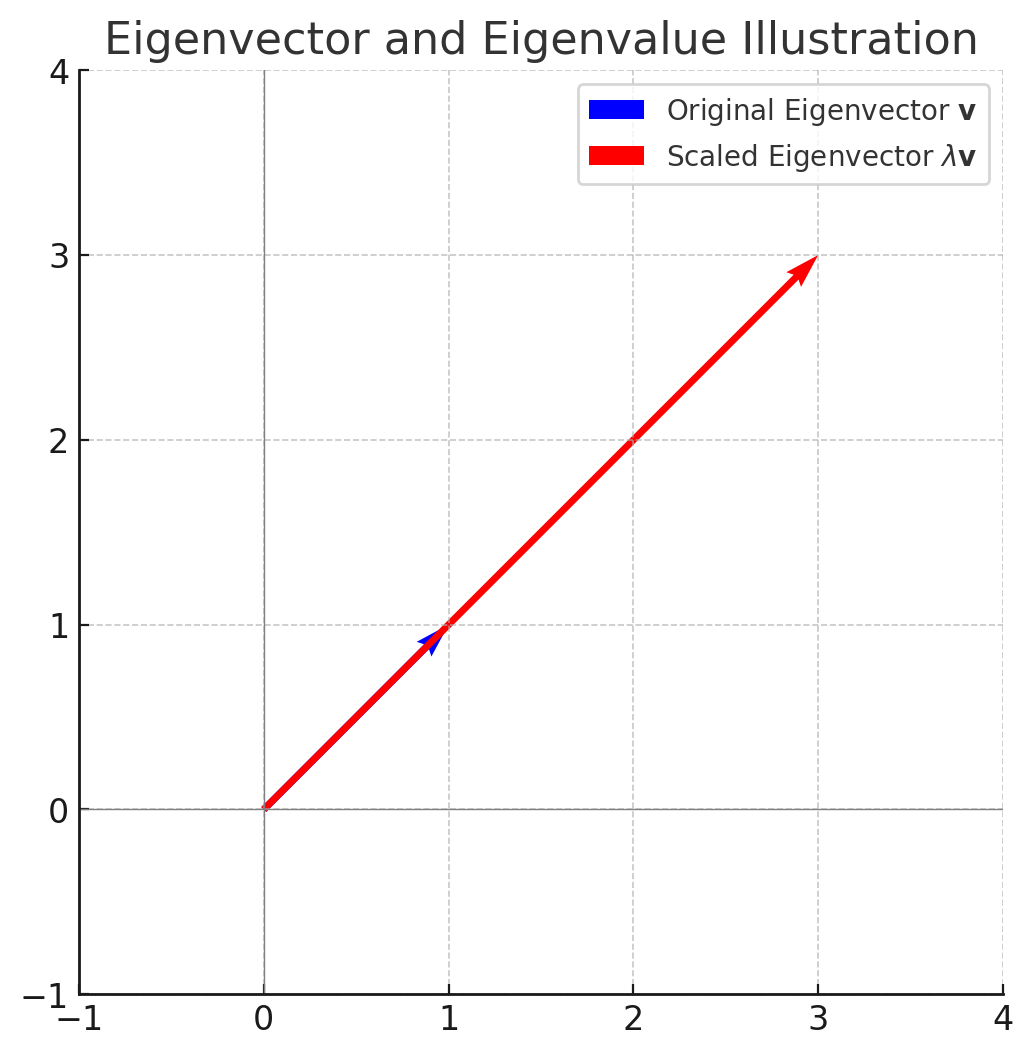
\includegraphics[width=0.35\textwidth]{eigenvector_plot.png}
\end{center}

\end{frame}


\begin{frame}{Asymptotic Behavior of Continuous-Time Systems}

Given a continuous-time linear system:
\[
x(t) = e^{A t} x(0),
\]
where \( A \) is diagonalizable, the initial state can be expressed as:
\[
x(0) = b_1 v_1 + b_2 v_2 + \dots + b_n v_n,
\]
where \( v_i \) are the eigenvectors of \( A \) and \( e^A \), and \( b_i \) are coefficients.

Applying this to the solution, we get:
\[
x(t) = b_1 e^{\lambda_1 t} v_1 + b_2 e^{\lambda_2 t} v_2 + \dots + b_n e^{\lambda_n t} v_n.
\]

\end{frame}

\begin{frame}{Summation of Exponential Terms}

So: the solution \( x(t) \) is a summation of multiple exponential terms:
\[
x(t) = b_1 e^{\lambda_1 t} v_1 + b_2 e^{\lambda_2 t} v_2 + \dots + b_n e^{\lambda_n t} v_n.
\]

\begin{itemize}
    \item \( \lambda_i \): Eigenvalues of \( A \).
    \item \( e^{\lambda_i t} \): Exponential growth or decay term corresponding to \( \lambda_i \).
    \item The absolute magnitude of each term is determined by \( |e^{\lambda_i t}| = e^{\mathrm{Re}(\lambda_i) t} \).
\end{itemize}

\end{frame}

\begin{frame}{Dominant Eigenvalue}

The term with the largest real part of \( \lambda_i \) dominates as \( t \to \infty \):

\[
|e^{\lambda_i t}| = e^{\mathrm{Re}(\lambda_i) t}.
\]

If \( \lambda_1 \) has the largest real part:
\[
\mathrm{Re}(\lambda_1) > \mathrm{Re}(\lambda_2), \, \mathrm{Re}(\lambda_3), \dots, \mathrm{Re}(\lambda_n),
\]
then as \( t \to \infty \):
\[
x(t) \approx e^{\lambda_1 t} b_1 v_1.
\]

\textbf{Key Insight:} The eigenvalue with the largest real part determines the system's asymptotic behavior.

\end{frame}

\begin{frame}{Role of Eigenvalues in System Dynamics}

An eigenvalue \( \lambda \) determines whether a system's state component (given by its corresponding eigenvector) grows, shrinks, or remains constant over time:

\begin{itemize}
    \item \(\mathrm{Re}(\lambda) > 0\): The component grows exponentially.
    \item \(\mathrm{Re}(\lambda) < 0\): The component shrinks exponentially.
    \item \(\mathrm{Re}(\lambda) = 0\): The component is conserved (no growth or decay).
\end{itemize}

For continuous-time models, the behavior of individual state components is tied to the real part of their eigenvalues.

\end{frame}

\begin{frame}{System Stability and the Dominant Eigenvalue}

The real part of the dominant eigenvalue \( \lambda_d \) determines the overall stability of a continuous-time system:

\begin{itemize}
    \item \(\mathrm{Re}(\lambda_d) > 0\): The system is \textbf{unstable}, diverging to infinity.
    \item \(\mathrm{Re}(\lambda_d) < 0\): The system is \textbf{stable}, converging to the origin.
    \item \(\mathrm{Re}(\lambda_d) = 0\): The system is \textbf{marginally stable}:
    \begin{itemize}
        \item The dominant eigenvector component is conserved.
        \item The system may converge to a non-zero equilibrium point.
    \end{itemize}
\end{itemize}

\textbf{Key Insight:} Stability is governed by the real part of the dominant eigenvalue \( \lambda_d \).

\end{frame}

\begin{frame}{Two-Dimensional Linear Dynamical System}

The "love affairs" model, proposed by Strogatz, is given as:

\[
\frac{dx}{dt} = 
\begin{pmatrix}
a & b \\
c & d
\end{pmatrix} x = A x, \quad A = 
\begin{pmatrix}
a & b \\
c & d
\end{pmatrix}.
\]

Key properties of the coefficient matrix \( A \) determine the system's stability:
\begin{itemize}
    \item Eigenvalues \( \lambda \) are critical to understanding the dynamics.
    \item Stability depends on the real part of the dominant eigenvalue \( \lambda_d \).
\end{itemize}

\end{frame}

\begin{frame}{Eigenvalue Calculation}

The eigenvalues \( \lambda \) of \( A \) are obtained by solving the characteristic equation:
\[
\det \begin{pmatrix}
a - \lambda & b \\
c & d - \lambda
\end{pmatrix} = 0.
\]

Simplifying:
\[
\lambda^2 - \mathrm{Tr}(A) \lambda + \det(A) = 0,
\]
where:
\begin{itemize}
    \item \( \mathrm{Tr}(A) = a + d \) (trace of \( A \)).
    \item \( \det(A) = ad - bc \) (determinant of \( A \)).
\end{itemize}

The eigenvalues are:
\[
\lambda_{\pm} = \frac{\mathrm{Tr}(A) \pm \sqrt{\mathrm{Tr}(A)^2 - 4 \det(A)}}{2}.
\]

\end{frame}

\begin{frame}{Dominant Eigenvalue}

The dominant eigenvalue is the one with the largest real part. Conditions:

\begin{itemize}
    \item If \( \mathrm{Tr}(A)^2 < 4 \det(A) \): The real part of \( \lambda \) is:
    \[
    \mathrm{Re}(\lambda_d) = \frac{\mathrm{Tr}(A)}{2}.
    \]
    \item If \( \mathrm{Tr}(A)^2 \geq 4 \det(A) \): The real part of \( \lambda \) is:
    \[
    \mathrm{Re}(\lambda_d) = \frac{\mathrm{Tr}(A) + \sqrt{\mathrm{Tr}(A)^2 - 4 \det(A)}}{2}.
    \]
\end{itemize}

The term with the \emph{plus} sign always dominates because it has the largest real part.

\end{frame}

\begin{frame}{Stability Diagram for Two-Dimensional Systems}

The stability of a two-dimensional linear dynamical system depends on the trace \( \mathrm{Tr}(A) \) and determinant \( \det(A) \) of the coefficient matrix \( A \).

\begin{itemize}
    \item \(\mathrm{Tr}(A)\): Sum of diagonal elements.
    \item \(\det(A)\): Determinant of the matrix.
\end{itemize}

\textbf{Stability Regions:}
\begin{itemize}
    \item \( \mathrm{Tr}(A) < 0 \, \text{and} \, \det(A) > 0 \): Stable system (converges to origin).
    \item \( \mathrm{Tr}(A) > 0 \): Unstable system (diverges).
    \item \( \det(A) < 0 \): Saddle point (unstable).
    \item \( \mathrm{Tr}(A)^2 < 4 \det(A) \): Complex eigenvalues (oscillatory behavior).
\end{itemize}

\end{frame}

\begin{frame}{Stability Diagram for Two-Dimensional Systems}
\begin{figure}[h]
    \centering
    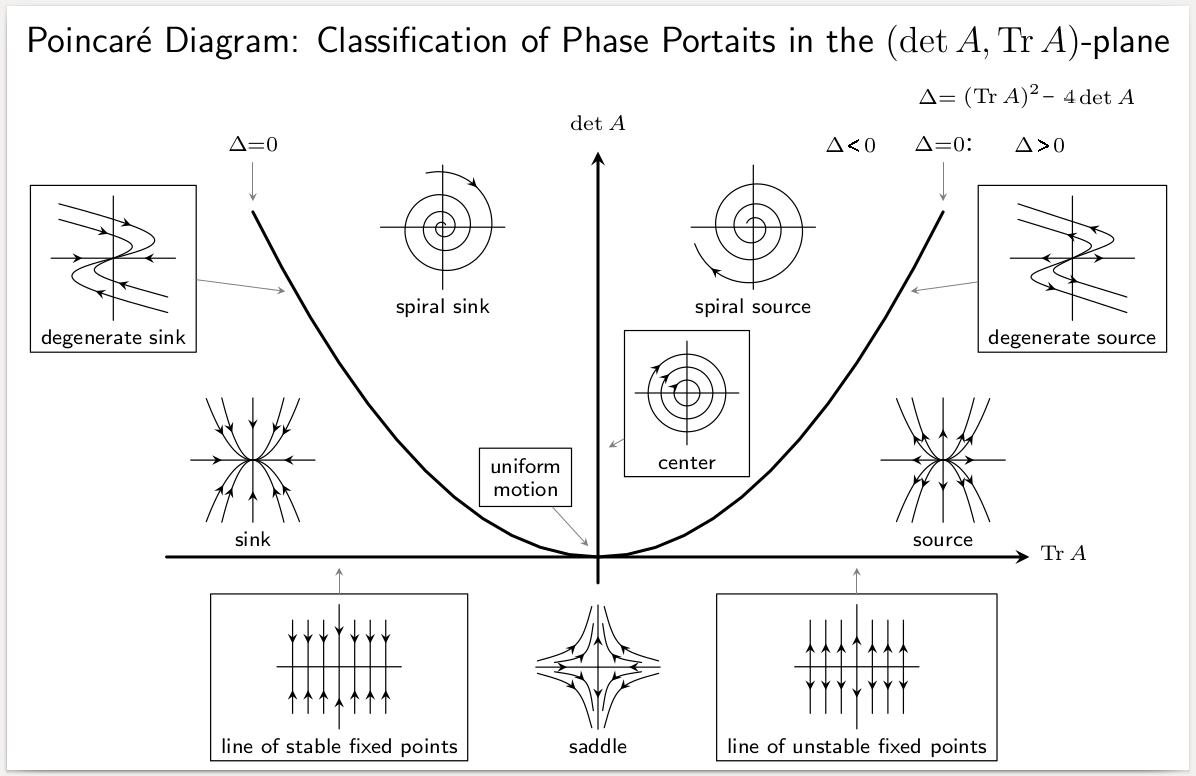
\includegraphics[width=0.6\textwidth]{Stability_Diagram-2.png}
    \caption{Stability Diagram. Credit: Freesodas, Wikimedia.}
\end{figure}

\scriptsize
\textbf{Note:} This diagram applies only to two-dimensional systems and is not generalizable to higher dimensions.
\end{frame}

\begin{frame}{Exercise: Stability Analysis}

Determine the stability of the following continuous-time linear systems:

\begin{enumerate}
    \item \( \frac{dx}{dt} = A x, \quad A = \begin{pmatrix} -1 & 2 \\ 2 & -2 \end{pmatrix}. \)
    \item \( \frac{dx}{dt} = A x, \quad A = \begin{pmatrix} 0.5 & -1.5 \\ 1 & -1 \end{pmatrix}. \)
\end{enumerate}

\textbf{Tasks:}
\begin{itemize}
    \item Find the eigenvalues of the system matrix \( A \).
    \item Analyze the real parts of the eigenvalues to determine stability.
\end{itemize}

\end{frame}

\begin{frame}{Solution to System 1}

For the first system:
\[
A = \begin{pmatrix} -1 & 2 \\ 2 & -2 \end{pmatrix}.
\]

\textbf{Step 1: Characteristic Equation}
\[
\det(A - \lambda I) = 0 \implies 
\det \begin{pmatrix} -1 - \lambda & 2 \\ 2 & -2 - \lambda \end{pmatrix} = 0.
\]

Simplify:
\[
(-1 - \lambda)(-2 - \lambda) - (2)(2) = 0.
\]
\[
\lambda^2 + 3\lambda = 0 \implies \lambda (\lambda + 3) = 0.
\]

\textbf{Eigenvalues:}
\[
\lambda_1 = 0, \quad \lambda_2 = -3.
\]

\end{frame}
\begin{frame}{Solution to System 1}

\textbf{Step 2: Stability Analysis}
\begin{itemize}
    \item \( \lambda_1 = 0 \): Marginally stable (eigenvalue on the imaginary axis).
    \item \( \lambda_2 = -3 \): Negative real part (stable).
\end{itemize}

\textbf{Conclusion:} The system is \textbf{marginally stable} because one eigenvalue is zero.

\end{frame}

\begin{frame}{Solution to System 2}

For the second system:
\[
A = \begin{pmatrix} 0.5 & -1.5 \\ 1 & -1 \end{pmatrix}.
\]

\textbf{Step 1: Characteristic Equation}
\[
\det(A - \lambda I) = 0 \implies 
\det \begin{pmatrix} 0.5 - \lambda & -1.5 \\ 1 & -1 - \lambda \end{pmatrix} = 0.
\]

Simplify:
\[
(0.5 - \lambda)(-1 - \lambda) - (-1.5)(1) = 0.
\]
\[
\lambda^2 + 0.5\lambda + 1 = 0.
\]

\end{frame}

\begin{frame}{Solution to System 2}

\textbf{Step 2: Solve for Eigenvalues}
\[
\lambda = \frac{-0.5 \pm \sqrt{(0.5)^2 - 4(1)(1)}}{2}.
\]
\[
\lambda = \frac{-0.5 \pm \sqrt{-3.75}}{2}.
\]
\[
\lambda = -0.25 \pm i\frac{\sqrt{3.75}}{2}.
\]

\textbf{Eigenvalues:}
\[
\lambda_1, \lambda_2 = -0.25 \pm i 0.968.
\]

\textbf{Step 3: Stability Analysis}
\begin{itemize}
    \item Real part of both eigenvalues is \( -0.25 \) (negative).
    \item The system is stable (converges to the origin).
\end{itemize}

\textbf{Conclusion:} The system is \textbf{stable}.

\end{frame}

\begin{frame}{Summary of Results}

The stability of the two systems is as follows:

\begin{enumerate}
    \item \( A = \begin{pmatrix} -1 & 2 \\ 2 & -2 \end{pmatrix} \):
    \begin{itemize}
        \item Eigenvalues: \( \lambda_1 = 0, \, \lambda_2 = -3 \).
        \item Stability: \textbf{Marginally stable} (zero eigenvalue).
    \end{itemize}

    \item \( A = \begin{pmatrix} 0.5 & -1.5 \\ 1 & -1 \end{pmatrix} \):
    \begin{itemize}
        \item Eigenvalues: \( \lambda = -0.25 \pm i 0.968 \).
        \item Stability: \textbf{Stable} (negative real part).
    \end{itemize}
\end{enumerate}

\textbf{Key Insight:} Stability depends on the real parts of the eigenvalues.

\end{frame}

\begin{frame}{Phase Space of Both Systems}

\begin{figure}[h]
    \centering
    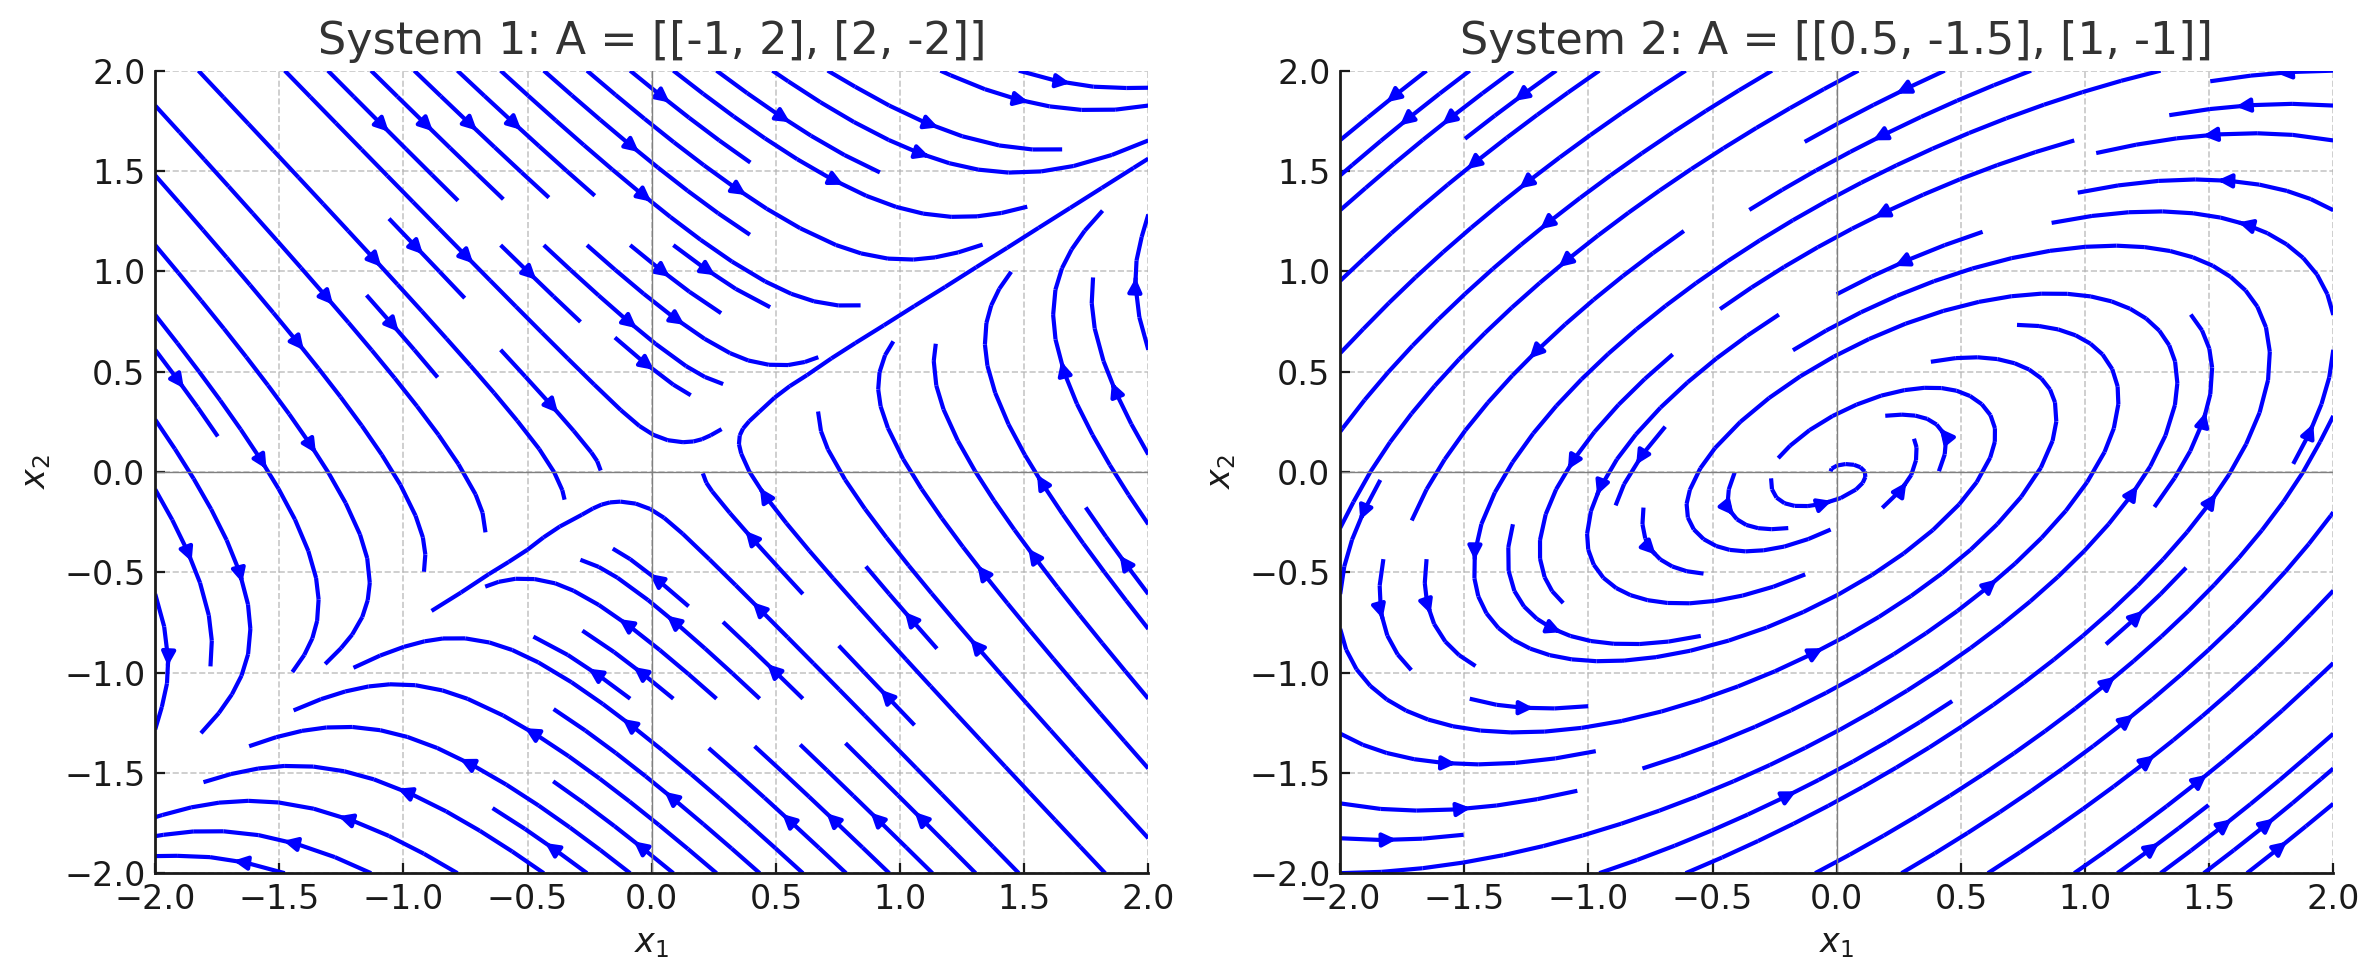
\includegraphics[width=0.75\textwidth]{phasespace_stability.png}
    \caption{Phase space of System 1 (left) and System 2 (right).}
\end{figure}
\scriptsize
\textbf{Observations:}
\begin{itemize}
    \item \textbf{System 1:} Shows marginal stability with trajectories moving toward a line due to the zero eigenvalue.
    \item \textbf{System 2:} Exhibits stable spiraling trajectories converging to the origin, indicating stability with complex eigenvalues.
\end{itemize}

\textbf{Key Insight:} Phase space visualizations clearly reveal the long-term behavior of the system states.

\end{frame}

\end{document}